\documentclass{article}
\usepackage{fullpage,amsmath,amsthm,graphicx,enumitem,amssymb}
\usepackage[hidelinks]{hyperref}
\theoremstyle{definition}
\newtheorem{thm}{Theorem}
\newtheorem{question}[thm]{Question}
\newenvironment{solution}{\noindent\textit{Solution:}}{}

\newcommand{\reals}{\mathbb{R}}

\title{ASEN 6519-007 Decision Making under Uncertainty\\
       Homework 5: Introduction to POMDPs}

\begin{document}

\maketitle

\section{Conceptual Questions}

\begin{question}
    Consider a modified version of the Crying Baby POMDP discussed in class and in Section 6.1.1 of \emph{Decision Making under Uncertainty} by Kochenderfer. This version is exactly as described in the book, except that the baby has a 20\% chance of becoming hungry at the next time step if it is not currently hungry and only a 60\% chance of crying when hungry. The alpha vectors for the optimal policy are shown below (green=\texttt{feed}, red=\texttt{don't feed}). The point at which the alpha vectors for feeding and not feeding intersect is at $P(\texttt{hungry}) = 0.19$. Draw an optimal policy graph with appropriate action and observation labels if the initial belief is certainty that the baby is not hungry ($b_0(\texttt{hungry}) = 0$)\footnote{On both of these problems, you are encouraged to use POMDPs.jl or other software packages}.

\begin{center}
    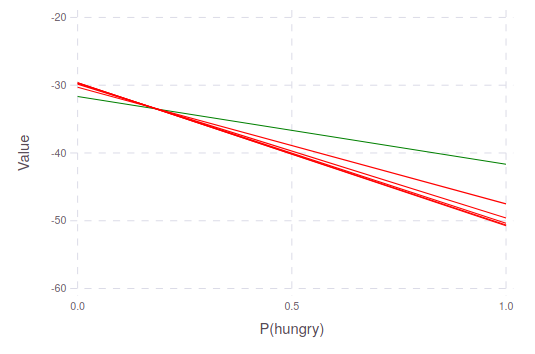
\includegraphics[width=0.7\textwidth]{alphas.png}
\end{center}

\end{question}

\pagebreak

\section{Exercises}

\begin{question}
    Consider the following POMDP that represents a personalized cancer monitoring plan\footnotemark[1]\footnote{Note that the probabilities are not meant to be realistic. See \url{https://pubsonline.informs.org/doi/10.1287/opre.1110.1019} for an actual publication on this topic}:

\begin{eqnarray*}
    \mathcal{S} &=& \left\{\texttt{healthy}, \texttt{in-situ-cancer}, \texttt{invasive-cancer}, \texttt{death}\right\}\\
    \mathcal{A} &=& \left\{\texttt{wait}, \texttt{test}, \texttt{treat}\right\}\\
    \mathcal{O} &=& \left\{\texttt{positive}, \texttt{negative}\right\}\\
    \gamma &=& 0.99\\
    s_0 &=& \texttt{healthy}
\end{eqnarray*}

The \textbf{transition dynamics} are as follows:
\begin{itemize}[noitemsep]
    \item If the patient is \texttt{healthy}, at each timestep, they have a 2\% chance of developing \texttt{in-situ-cancer}.
    \item If the patient has \texttt{in-situ-cancer} and they are \texttt{treat}ed, they have an 60\% chance of becoming healthy at the next time step.
    \item If the patient has \texttt{in-situ-cancer} and they are not \texttt{treat}ed, they have a 10\% chance of developing \texttt{invasive-cancer}.
    \item If the patient has \texttt{invasive-cancer} and they are \texttt{treat}ed, they have a 20\% chance of recovering and a 20\% chance of dying at the next time step.
    \item If the patient has \texttt{invasive-cancer} and they are not \texttt{treat}ed, they have a 60\% chance of dying.
    \item In all other cases, the state remains the same as in the previous step.
\end{itemize}

The \textbf{observation} is determined as follows:
\begin{itemize}[noitemsep]
    \item If the action is \texttt{test} and the \emph{new} state is \texttt{healthy}, then the observation will be (falsly) \texttt{positive} 5\% of the time. 
    \item If the action is \texttt{test} and the \emph{new} state is \texttt{in-situ-cancer} then the observation will be \texttt{positive} 80\% of the time.
    \item If the action is \texttt{test} and the \emph{new} state is \texttt{invasive-cancer} then the observation will be \texttt{positive}.
    \item If the action is \texttt{treat} and the \emph{new} state is \texttt{in-situ-cancer} or \texttt{invasive-cancer} then the observation will be \texttt{positive}.
    \item In all other cases, the observation is \texttt{negative}.
\end{itemize}

The \textbf{rewards} are defined as follows (one could interpret the reward as roughly quality years of life):
\begin{itemize}[noitemsep]
    \item $R(\texttt{death}, \text{any action}) = 0.0$ (i.e. \texttt{death} is a terminal state)
    \item $R(\text{any living state}, \texttt{wait}) = 1.0$
    \item $R(\text{any living state}, \texttt{test}) = 0.8$ (because of costs and anxiety about a positive result)
    \item $R(\text{any living state}, \texttt{treat}) = 0.1$
\end{itemize}

\begin{enumerate}[label=(\alph*)]
    \item Use Monte Carlo simulations to evaluate a policy that always \textbf{wait}s.
    \item Propose a better heuristic strategy based on the observation history or belief and evaluate it with Monte Carlo simulations. See if you can get an average discounted return of 75 or more.
\end{enumerate}

\end{question}

\end{document}
